%*****************************************
\chapter{3D Spieleentwicklung mit Java}\label{ch:beispiele}
%*****************************************

\section{Allgemeiner Aufbau von 3D Spielen}\label{sec:aufbau}

Bei 3-dimensionalen Spielen wird das Spielgeschehen in einen Raum transferiert und dem Spieler die Möglichkeit gegeben sich dort frei bewegen zu können. \newline
Im Gegensatz zu 2-dimensionalen Spielen sind hier deutlich mehr Berechnungen auf vektorieller Ebene notwendig, was sich auf die Laufzeit niederschlägt. Daher ist es besonders wichtig ein effizientes Programm zu generieren.
Diesbezüglich ist Java nicht die optimale Programmiersprache, da durch den Interpreter viel Zeit verloren geht.
\linebreak
Im Allgemeinen kann man sagen, dass die meisten 3D Spiele folgende Elemente enthalten:
\begin{itemize}
	\item 3D-Modelle und eine räumliche Spielumgebung
	\item Eine sog. "Kamera", welche nur den relevanten Teil des Bildes abbildet
	\item Möglichkeiten der Interaktion
\end{itemize}



\bigskip
https://de.wikipedia.org/wiki/Spiel-Engine





\section{Funktionsweise und Auswahl von Game Engines}\label{sec:jMonkeyEngine}
Um nicht sämtliche mathematischen Berechnungen auf der Grafikkarte selber programmieren, oder beispielsweise die Lautsprecher für Audio-Effekte ansprechen zu müssen, erhält der Entwickler Unterstützung durch sogenannte "Game Engines".
Diese beinhalten die Basisfunktionen von Spielen und ermöglichen dem Spiele-Programmierer eine gezieltere Entwicklung. Zu den Basisfunktionalitäten gehören im Allgemeinen die folgenden:
\begin{enumerate}
	\item Grafik-Engine
	\item Physiksystem
	\item Soundsystem
	\item Zustandsspeicherung
	\item Steuerung
	\item Datenverwaltung
\end{enumerate}
Zur Auswahl stehen eine Vielzahl von verschiedenen Engines, welche jeweils vor und Nachteile mit sich bringen. Da wir auf jeden Fall lernen wollten, wie die grundlegenden Dinge funktionieren, haben wir nach Engines gesucht, welche nur die Basisfunktionalitäten unterstützen, jedoch keine automatische Codegenerierung, Drag and Drop oder Editoren beinhalten.
Im folgenden eine Übersicht einiger Engines:


\begin{table}
	\myfloatalign
	\begin{tabularx}{\textwidth}{Xll} \toprule
		\tableheadline{GameEngine} & \tableheadline{Vorteile} & \tableheadline{Nachteile} \\ \midrule 
		Unity & Sehr bekannt, beliebt &  zu oberflächlich, kein Java \\
		jMonkeyEngine & Sehr entwicklungsnahe, Java & Schlechte Dokumentation \\
		Wurfel Engine & Sehr benutzerfreundlich & keine Physikunterstützung \\
		\bottomrule
	\end{tabularx}
	\caption[Engines]{Vor und Nachteile einiger Game Engines}  \label{tab:example}
\end{table}

\bigskip
Letztendlich fiel die Entscheidung auf die jMonkeyEngine, welche häufig von Java Entwicklern verwendet wird. 

https://de.wikipedia.org/wiki/Spiel-Engine
https://de.wikipedia.org/wiki/Liste-von-Spiel-Engines


\subsection {Die jMonkeyEngine}
Die jMonkeyEngine (jME) ist komplett in Java geschrieben und basiert auf dem Buch "3D Game Engine Design" von David Eberly.
Durch eine Abstraktionsschicht kann jedes beliebige Rendering System verwendet werden, beispielsweise die Lightweight Java Game Library (LWJGL) oder die Open Graphics Library (OpenGL).
Die neuste Version ist jME3, welche einige hilfreiche Funktionen mit sich bringt, wie z.B. ein Partikelsystem, Frustum Culling oder 3D Sound Unterstützung.


https://de.wikipedia.org/wiki/JMonkeyEngine


\section{Umsetzung in Programmcode}\label{sec:code}
Im folgenden wird beschrieben wie einzelne Elemente in der jMonkeyEngine programmiert werden können und was dabei zu beachten ist.

https://docs.jmonkeyengine.org/beginner/beginner-intro.html

\subsection{Erzeugung der Application-Klasse: SimpleApplication}
Die Main-Klasse jedes jME3 Spieles erbt von der Klasse SimpleApplication, welche ein Spiel darstellt.
In der main-Methode wird dann eine neue Instanz erstellt und anschließend gestartet.

Jede Unterklasse der SimpleApplication beinhaltet diese Methoden:
\begin{enumerate}
	\item simpleInitApp():
	Sorgt für das Laden von Modellen, der Erstellung einer räumlichen Umgebung sowie jegliche Initiierungen.
	\item simpleUpdate(float tpf):
	Wird jedes frame per second (fps) ausgeführt und kümmert sich um gegebenenfalls neue Zustände.
	\item simpleRender(RenderManager rm):
	Wird stets nach simpleUpdate aufgerufen und zeichnet das Sichtbild des Spielers neu. Dazu bekommt die Methode einen RenderManager übergeben, welcher Präferenzen beim Zeichnen berücksichtigt (z.B. welche Ebene vorne oder hinten ist).
\end{enumerate}

Die erste der drei Methoden wird stets zu Beginn ausgeführt um alle benötigten Elemente bereit zu stellen.

\subsection{Funktionsweise von Nodes}
Um Elemente zum Renderingprozess hinzuzufügen, um sie also sichtbar zu machen, müssen diese an ensprechende "Nodes" (Knoten) angehängt werden.
Hierbei gibt es je nach Verwendungszweck verschiedene Arten zum Beispiel audioNode für Soundobjekte oder guiNode für Elemente auf der Benutzeroberfläche.
Zuletzt werden alle Nodes an die rootNode, also die Wurzel, angehängt. Im  Programmcode funktioniert dies mit der Methode attach() bzw. detach() zum entfernen.
Selbstverständlich können Objekte auch direkt an die rootNode angehängt werden.
Allerdings ist es empfehlenswert eine geeignete Baumstruktur zu erstellen um so bestimmte Elemente in Gruppen anzusprechen.
\bigskip
Beispiel: Erzeugung einer eigenen Node durch:
\begin{center}
	\fcolorbox{grau}{grau}{Node myNode = new Node();}
\end{center}

Wird nun beispielsweise die folgende Funktion auf dem Konten ausgeführt,
\begin{center}
	\fcolorbox{grau}{grau}{myNode.doSomething();}	
\end{center}

so wird diese auch für sämtliche Kinder des Knotens ausgeführt.


\subsection{Modelle und Assets}
Sämtliche externe Gegenstände des Spiels werden im assets Ordner im jME3 Projekt gesammelt. Dies sind multi-media Dateien wie 3D-Modelle, Soundfiles, Texturen, Shader und was sonst noch benötigt wird.
Um diese dann aus dem Ordner ins Spiel zu laden wird der sogenannte AssetManager benötigt, welcher einfach eine Instanz der Klasse mit entsprechenden Funktionalitäten ist.
Modelle sind dreidimensionale Gebilde welche verschiedenste Elemente in einem Spiel sein können. Hierbei verwendet jME3 die Klasse Spatial (engl. für "räumlich"). 

Zum Laden eines Objektes wird die entsprechende Funktion loadTexture() aufgerufen und der entsprechende Pfad zum Modell übergeben.

\begin{center}
\fcolorbox{grau}{grau}
{Spatial baum = assetManager.loadTexture("Models/Baum.j3o");}
\end{center}

Für Modelle gibt es viele verschiedene Datentypen. Neben dem jMonkey-eigenen Dateiformat j3o existieren unter anderem folgende wichtige Vertreter:
\begin{enumerate}
	\item XML-Dateien: Aus mesh.xml Daten wird ein Objekt erzeugt. 
	\item OBJ-Dateien: Die allgemeine Darstellung für Objekte.
	\item Blender-Dateien: Dies sind Dateien aus der Blender-Software, mit welcher Modelle erzeugt werden können.
\end{enumerate}

\bigskip
Um Modelle sichtbar zu machen müssen diese nun nur noch zu einer Node z.B. der rootNode hinzugefügt werden. 

\begin{center}
	\fcolorbox{grau}{grau}
	{rootNode.attachChild(baum);}
\end{center}


Neben dem Polygonzug und dem Material gibt es noch das Skelett. Dieses kann ebenfalls in einem entsprechenden Programm wie Blender erzeugt werden und daraus bestimmte Bewegungsabläufe in Spielen bestimmt werden.
Das Skelett ist notwendig für Animationen von Modellen wie beispielsweise Gehen, Springen oder Ähnliches.
In unserem Spiel haben wir uns für eine First-Person Perspektive entschieden, wodurch keine Animationen für den Spieler notwendig waren.



\subsection{Materialien}
Ein Modell besteht im Allgemeinen aus drei wichtigen Elementen.
Die Hauptstruktur (Polygonzug), das Skelett (Bewegungsapparat) und dann noch das Material.
Letzteres bestimmt wie das Modell aussieht, d.h. welche Farben und Strukturen das Modell an den entsprechenden Stellen bekommt.
Dateien für das Material sind meist test.material aber auch Bilddateien wie test.jpg oder test.png sind gängig.


\begin{figure}[h]
	\myfloatalign
	\subfloat[Modell ohne Material]
	{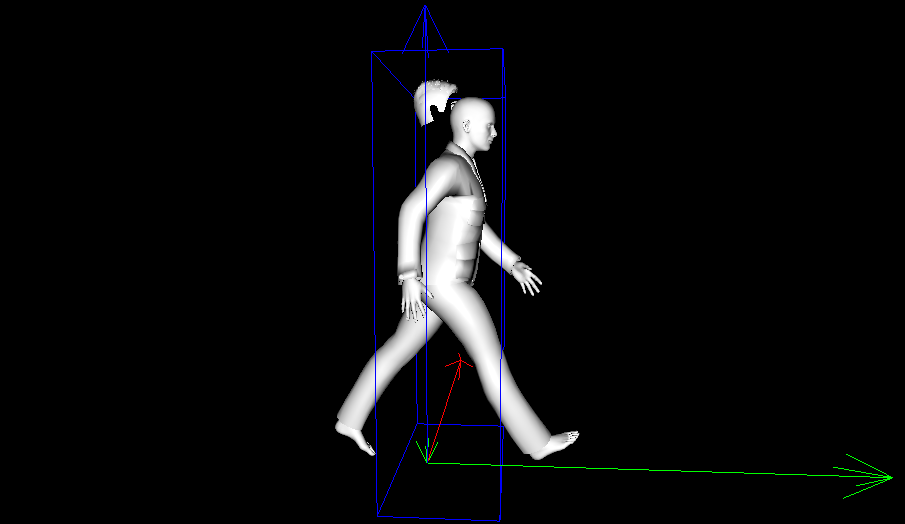
\includegraphics[width=.45\linewidth]{images/modelmat}} \quad
	\subfloat[Modell mit Material]
	{\label{fig:example-b}%
		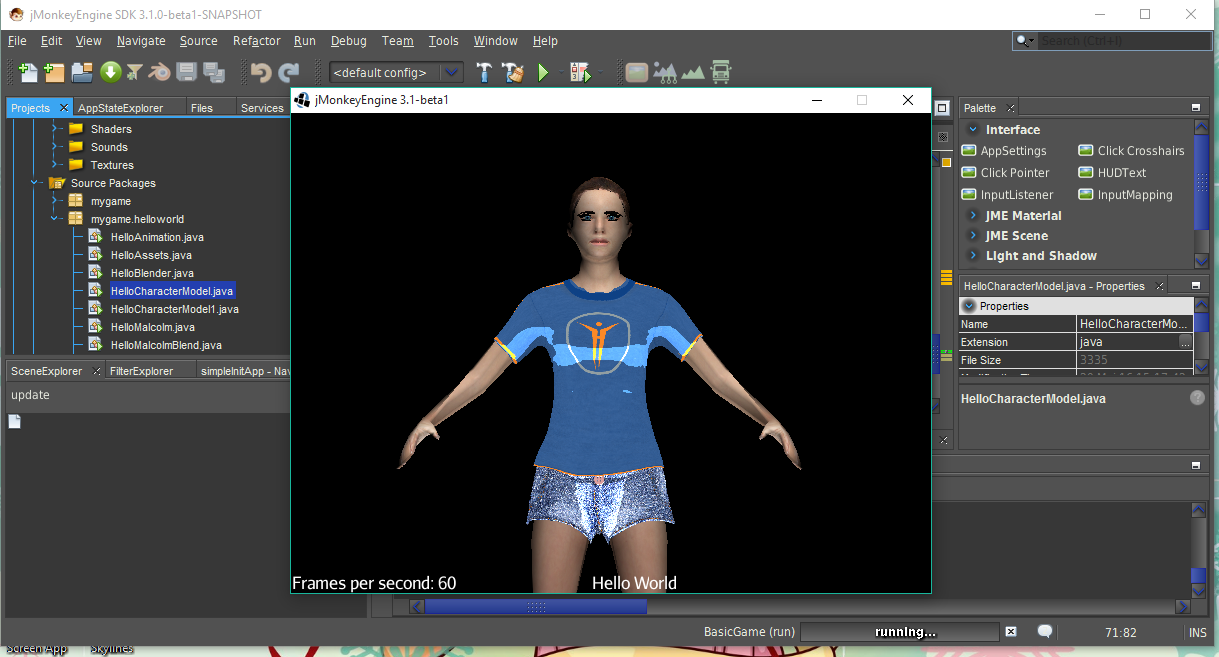
\includegraphics[width=.45\linewidth]{images/modelmat2}} \\
	\caption[Bilder.]{Modell mit und ohne Material}\label{fig:example}
\end{figure}

\bigskip

https://hub.jmonkeyengine.org/t/changes-to-animations-loading-in-blender-importer-important-for-importer-users/28304/10



\subsection{User-Input}

Aus einem 3-dimensionalen Gebilde wird erst dann ein Spiel, wenn Interaktion mit dem Spieler stattfindet. Dazu müssen Tasteneingaben, Mauseingaben oder gegebenfalls auch Toucheingaben abgefangen und verarbeitet werden.
Hierbei werden die bekannten Listener-Klassen verwendet.
TODO:
Welche möglichkeiten zur Spiel/Shoot/Jump usw Bewegung abgefangen werden sollten.
Dann natürlich Listener Klassen und wie FirstPerson gesteuert werden kann.

\subsection{Kollisionserkennung}
Allgemeine Beschreibung mit mesh als Form für die Kollision. Dann natürlich wie die Kollision funktioniert (aufruf von Methoden overlap, dann nicht weiter...)
Wird intern von jme3 übernommen und kann auch direkt im scene composer verwendet werden.

\subsection{Erzeugung einer Spielumgebung}
Terrain oder SceneComposer, sky, 
Funktionalität und allgemeines vorgehen.

\subsection{Hinzufügen von Audio}

\subsection{Physikalische Modellierung}
Allgemeines zu Gravity, usw... wird von jme3 unterstützt.

\subsection{Effekte und Details}

\subsubsection{Nebel}
\begin{eqnarray*} \xi  = \frac{2\pi z^2 e^4 N_{\textrm{Av}} Z \rho
		\delta x}{m_{\textrm{e}} \beta^2 c^2 A} =  153.4 \frac{z^2}{\beta^2}
	\frac{Z}{A}
	\rho \delta x \quad\textrm{keV},
\end{eqnarray*}
\bigskip
\begin{equation}
\kappa =\frac{\xi}{E_{\textrm{max}}} %\mathbb{ZNR}
\end{equation}


\[
E_{\textrm{max}} =\frac{2 m_{\textrm{e}} \beta^2\gamma^2 }{1 +
	2\gamma m_{\textrm{e}}/m_{\textrm{x}} + \left ( m_{\textrm{e}}
	/m_{\textrm{x}}\right)^2}\ ,
\]

\subsubsection{Partikeleffekte}
Feuer, Regen... usw...


\section{Optimierung des Programms}\label{sec:optimizing}
Erklärung mit Rendering (Fragment/Vertex), dass sehr viele Dreiecke berechnet werden und dadurch die FPS im Keller sind. Erklärung von Möglichkeiten zur Optimierung.
Hinweis dass es bei 3D spielen zwingend notwending ist zu optimieren...

\subsubsection{Minimierung der Anzahl von Modellen}
\subsubsection{Level of Detail (LOD)}
Das ist ein Zitat. \cite{Wa14b}.
\begin{description}
	\item[Begriff A:] Und so funktioniert eine Begriffsbeschreibung.
\end{description}









\begin{table}
	\myfloatalign
	\begin{tabularx}{\textwidth}{Xll} \toprule
	\tableheadline{jMonkeyEngine} & \tableheadline{Vorteile} & \tableheadline{Nachteile} \\ \midrule 
    Dokumentation & viele Beispiele &  oft deprecated \\
	Noch ein Punkt & Julian & Florian \\
	\bottomrule
	\end{tabularx}
	\caption[Kurzer Titel Tabelle.]{Beispiel für eine Tabelle}  \label{tab:example}
\end{table}



\begin{figure}[bth]
        \myfloatalign
        \subfloat[Asia personas duo.]
        {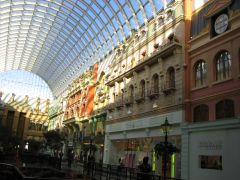
\includegraphics[width=.45\linewidth]{images/example_1}} \quad
        \subfloat[Pan ma signo.]
        {\label{fig:example-b}%
         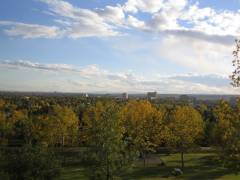
\includegraphics[width=.45\linewidth]{images/example_2}} \\
        \subfloat[Methodicamente o uno.]
        {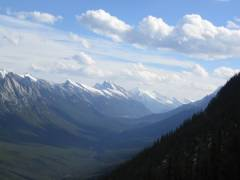
\includegraphics[width=.45\linewidth]{images/example_3}} \quad
        \subfloat[Titulo debitas.]
        {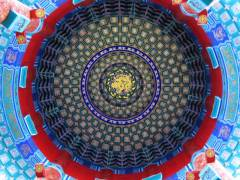
\includegraphics[width=.45\linewidth]{images/example_4}}
        \caption[Bilder.]{Beispielbilder von jMonkey.}\label{fig:example}
\end{figure}






